\section{Вычислительный эксперимент}\label{sec4}

Проводится эксперимент для анализа свойств предложенных методов оценки достаточного размера выборки. Эксперимент состоит из двух частей. В первой части рассматриваются оценки достаточного размера выборки в случае, когда достаточный размер выборки не превосходит доступный. Во второй части исследуются результаты, полученные в условиях того, что достаточный размер выборки больше доступного.

\subsection{Достаточный размер выборки не превосходит доступный}

Синтетические данные сгенерированы из модели линейной регрессии. Число объектов 1000, число признаков 20. Далее приведены графики логарифма функции правдоподобия выборки, а также функций $D(k)$ и $M(k)$, определенных в Главе~\ref{sec2} (здесь используется логарифм функции правдоподобия). Выполнено определение D-достаточного и M-достаточного размеров выборки. Использовалось $B=1000$ бутстрап-выборок. Результаты представлены на Рис.~\ref{synthetic-regression-sufficient}.

\begin{figure}[h!]
    \centering
    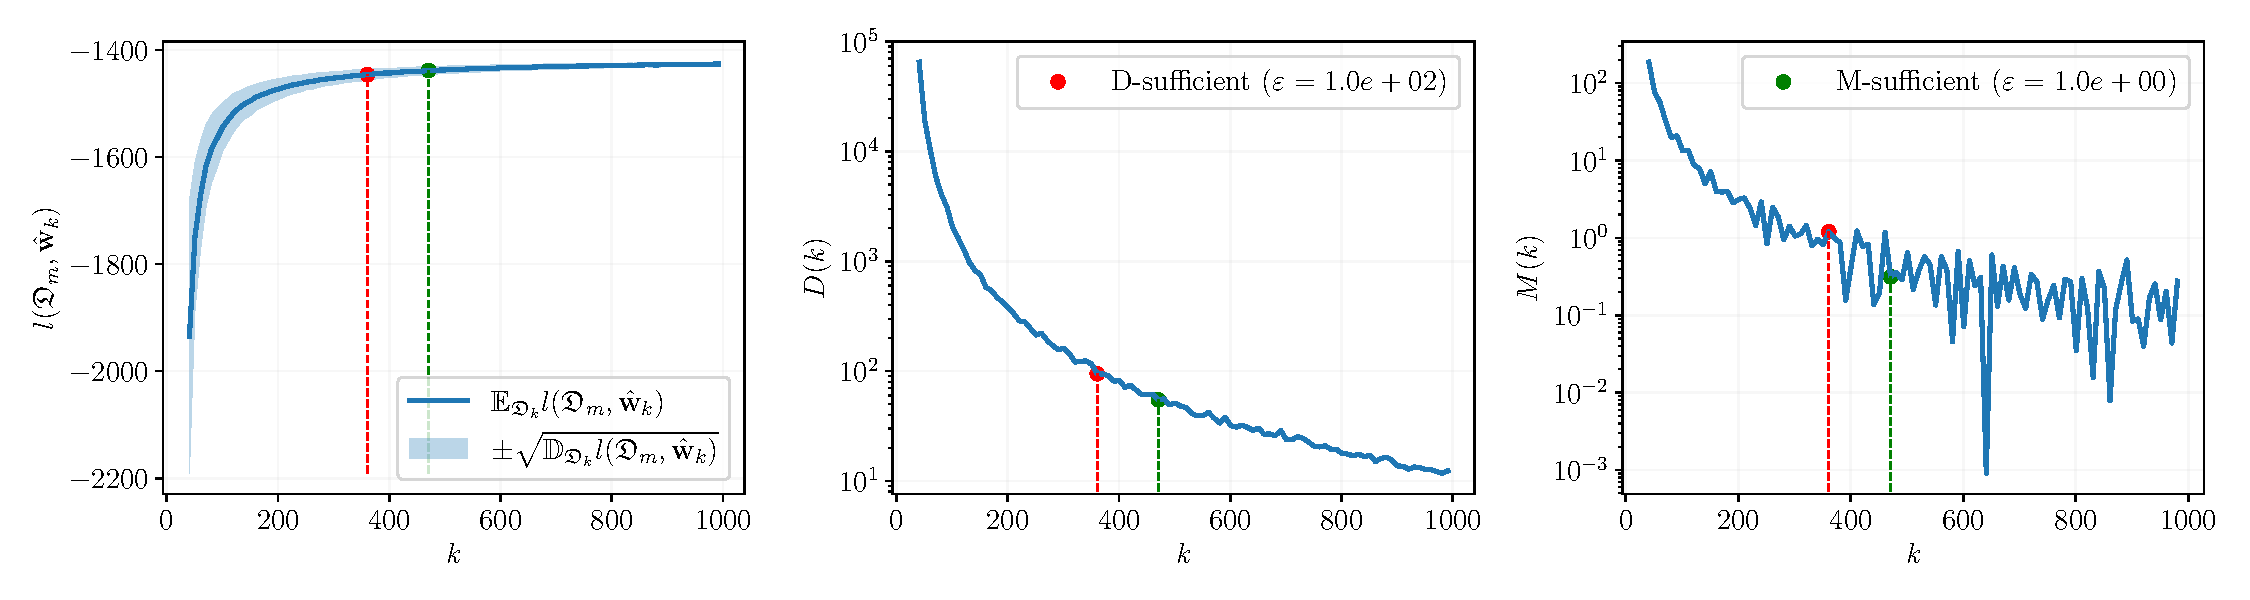
\includegraphics[width=\textwidth]{figures/synthetic-regression-sufficient.pdf}
    \caption{Синтетическая выборка (линейная регрессия) при $m^* \leqslant m$}
    \label{synthetic-regression-sufficient}
\end{figure}

Вторая синтетическая выборка сгенерирована из модели логистической регрессии. Число объектов 1000, число признаков 20. Аналогичные графики приведены на Рис.~\ref{synthetic-classification-sufficient}.

\begin{figure}[h!]
    \centering
    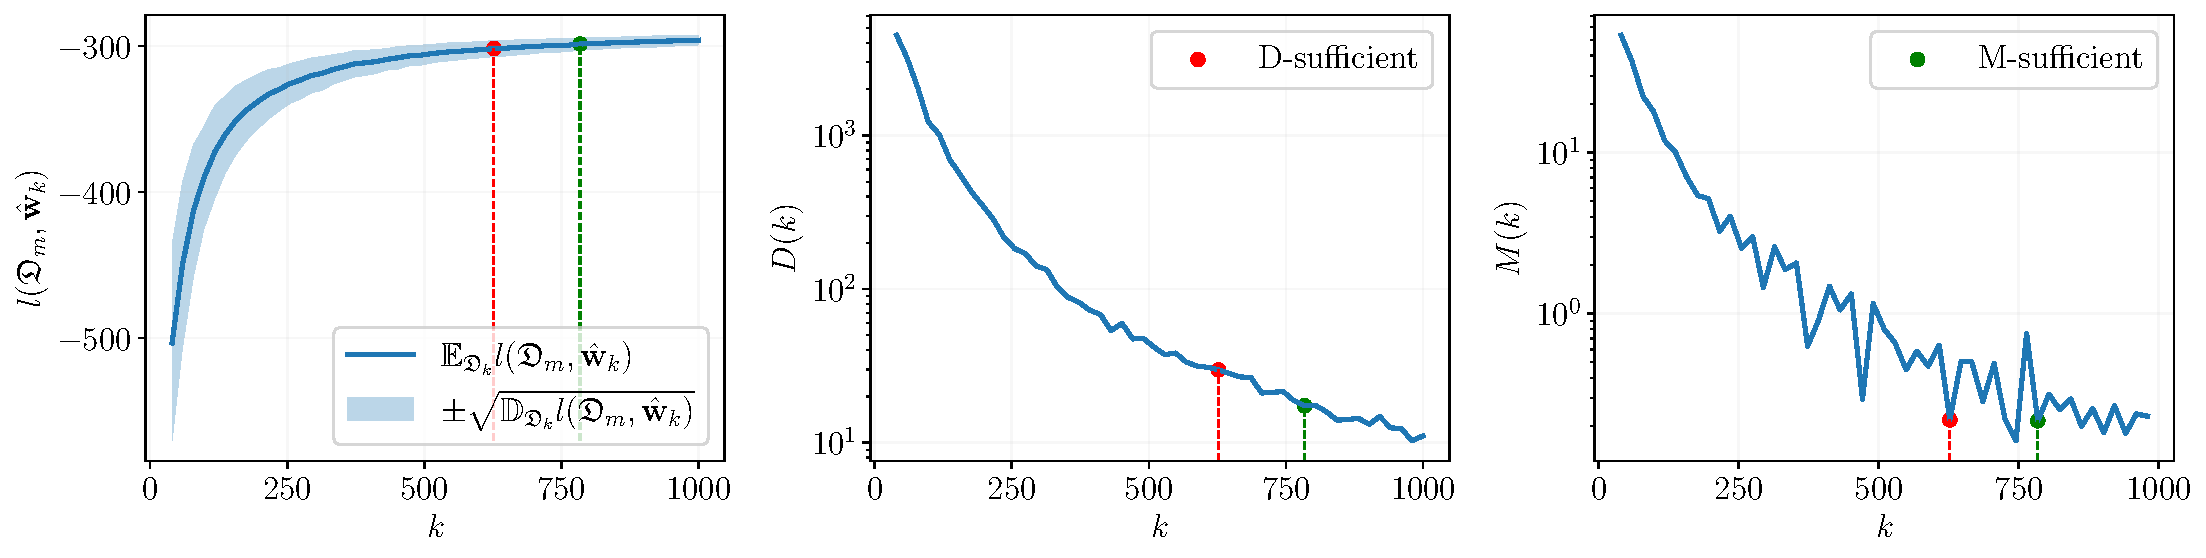
\includegraphics[width=\textwidth]{figures/synthetic-classification-sufficient.pdf}
    \caption{Синтетическая выборка (логистическая регрессия) при $m^* \leqslant m$}
    \label{synthetic-classification-sufficient}
\end{figure}

\subsection{Достаточный размер выборки больше доступного}

Для синтетических выборок проведена аппроксимация функций правдоподобия. Среднее значение и дисперсия аппроксимированы соответственно функциями
\[ \varphi(m) = a_1 - a_2^2 \exp\left( - a_3^2 m \right) - \dfrac{a_4^2}{m^{3/2}} \]
и
\[ \psi(m) = b_1^2 \exp\left( - b_2^2 m \right) + \dfrac{b_3^2}{m^{3/2}}, \]
где $\mathbf{a}$ и $\mathbf{b}$~--- вектора параметров.

Производилось разделение на обучающую и тестовую выборки в соотношении 70:30. Аппроксимация производилась только на обучающей части. Достаточный размер выборки находился в тестовой части. На Рис.~\ref{synthetic-regression-approximation} и Рис.~\ref{synthetic-classification-approximation} представлены истинные и восстановленные зависимости. Там же указаны определенные D-достаточный и M-достаточный размеры выборки.

\begin{figure}[h!]
    \centering
    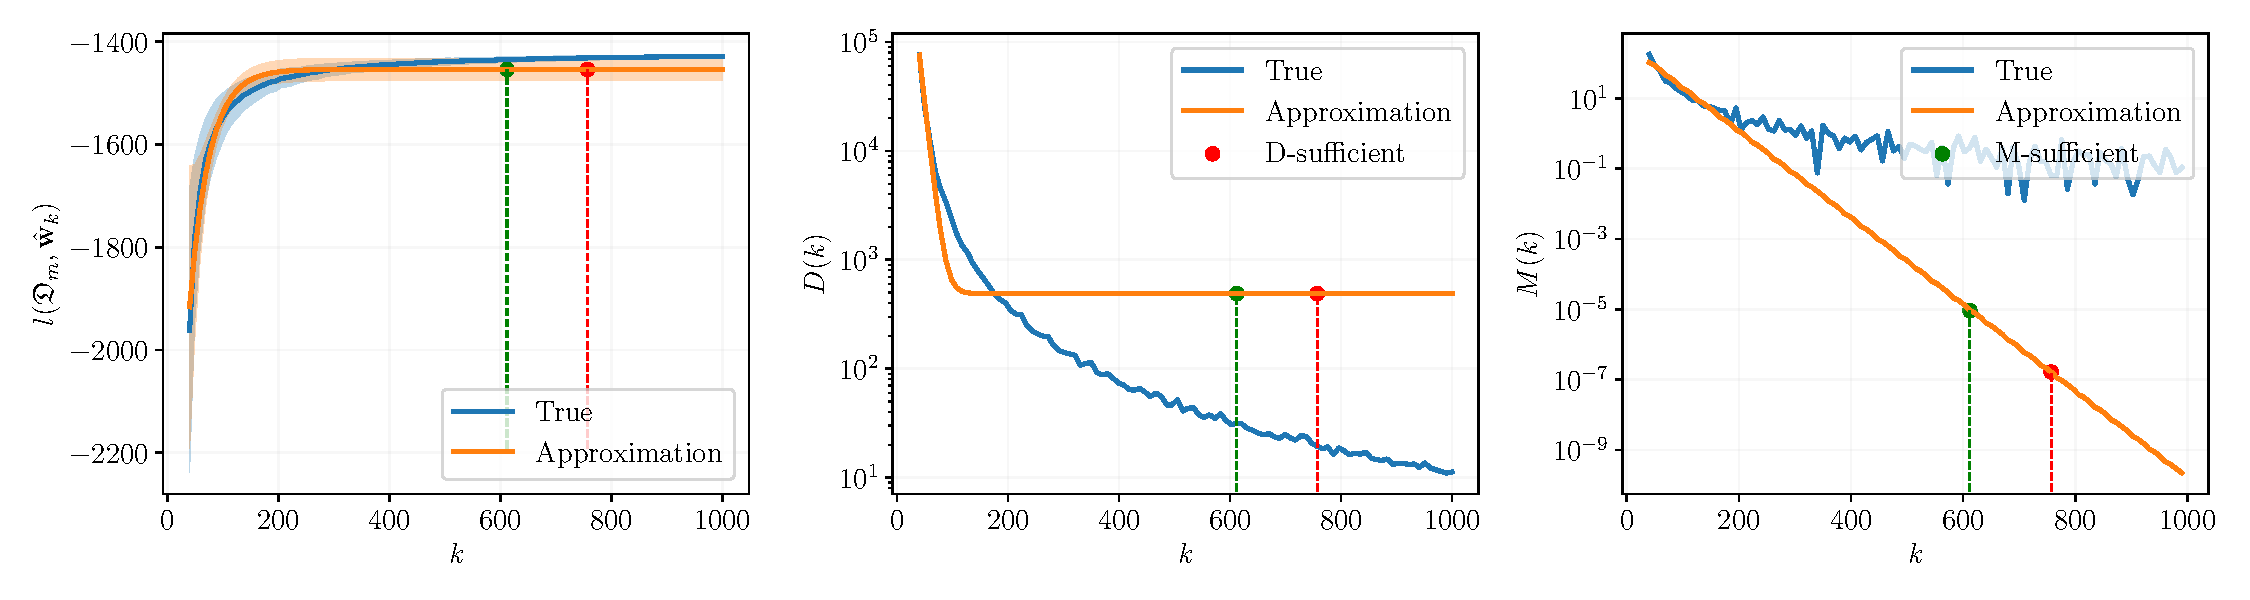
\includegraphics[width=\textwidth]{figures/synthetic-regression-approximation.pdf}
    \caption{Синтетическая выборка (линейная регрессия) при $m^* > m$}
    \label{synthetic-regression-approximation}
\end{figure}

\begin{figure}[h!]
    \centering
    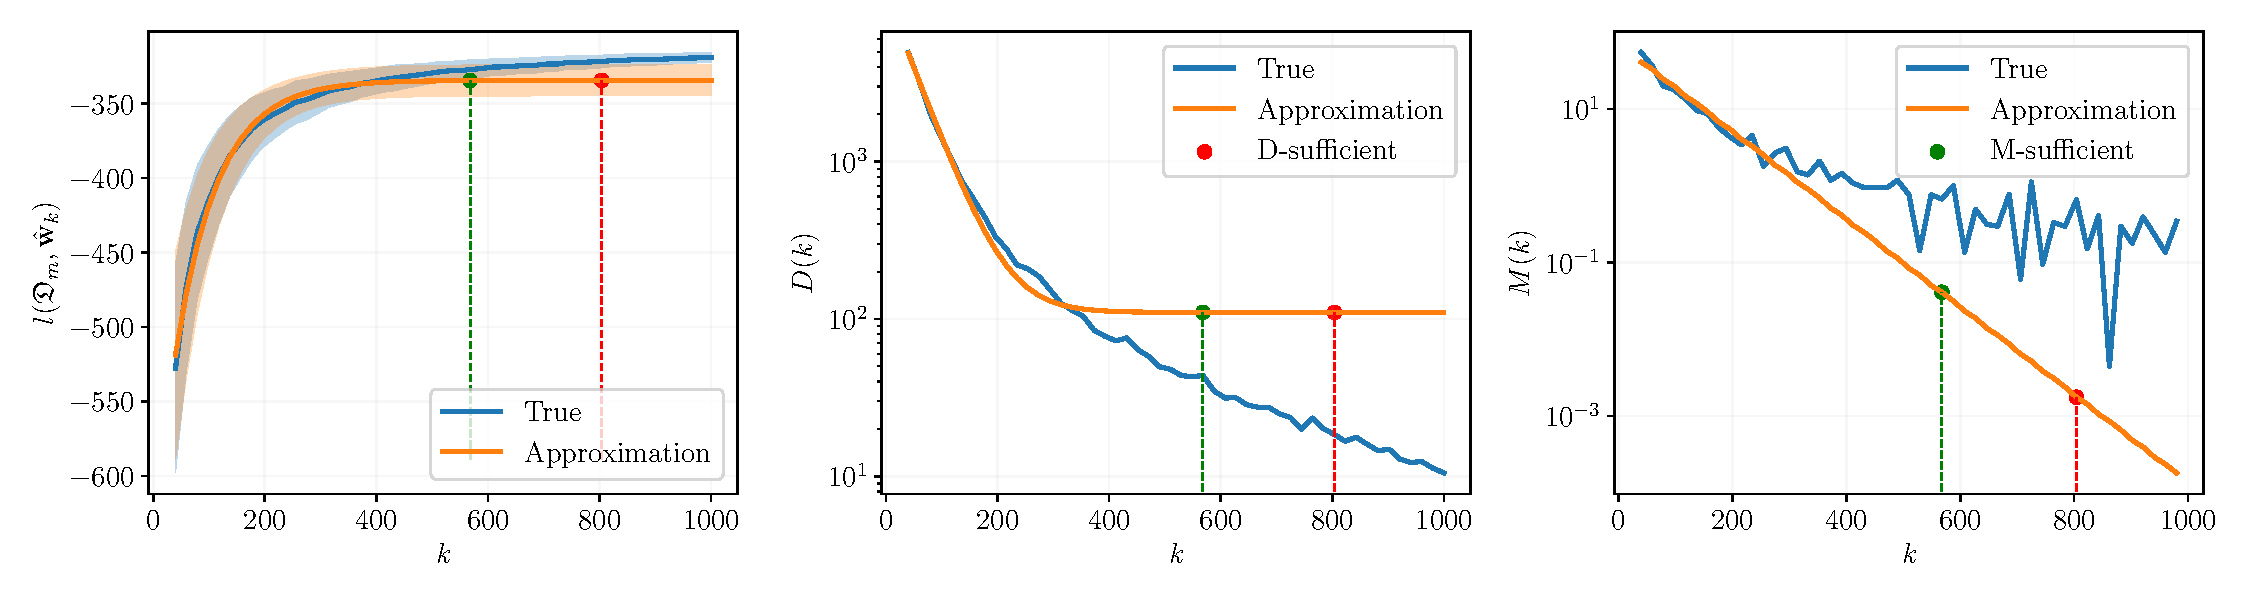
\includegraphics[width=\textwidth]{figures/synthetic-classification-approximation.pdf}
    \caption{Синтетическая выборка (логистическая регрессия) при $m^* > m$}
    \label{synthetic-classification-approximation}
\end{figure}